

\paragraph{}The overall structure of the system is designed to seamlessly support the palletizing task utilizing the UR20 robot arm and PLC. At the core of the system is the Programmable Logic Controller (3PE Teaching Pendant), which orchestrates all operations by receiving inputs from various sensors and executing predefined routines for box handling. The data flow begins with the conveyor belt layer, transporting boxes to be distributed on the pallet, which are indicated as ready by the Photo Eye sensor that will relay information to the PLC to move onto the next part of the routine, given it detects a box incoming. The Safety Sensor Layer regulates movement detects human presence to dynamically adjust or halt movement as needed, ensuring a safe operating environment. The UR20 Arm Layer is responsible for picking up and placing boxes using a vacuum gripper and movement control system, all based on commands from the PLC.

\begin{figure}[h!]
	\centering
 	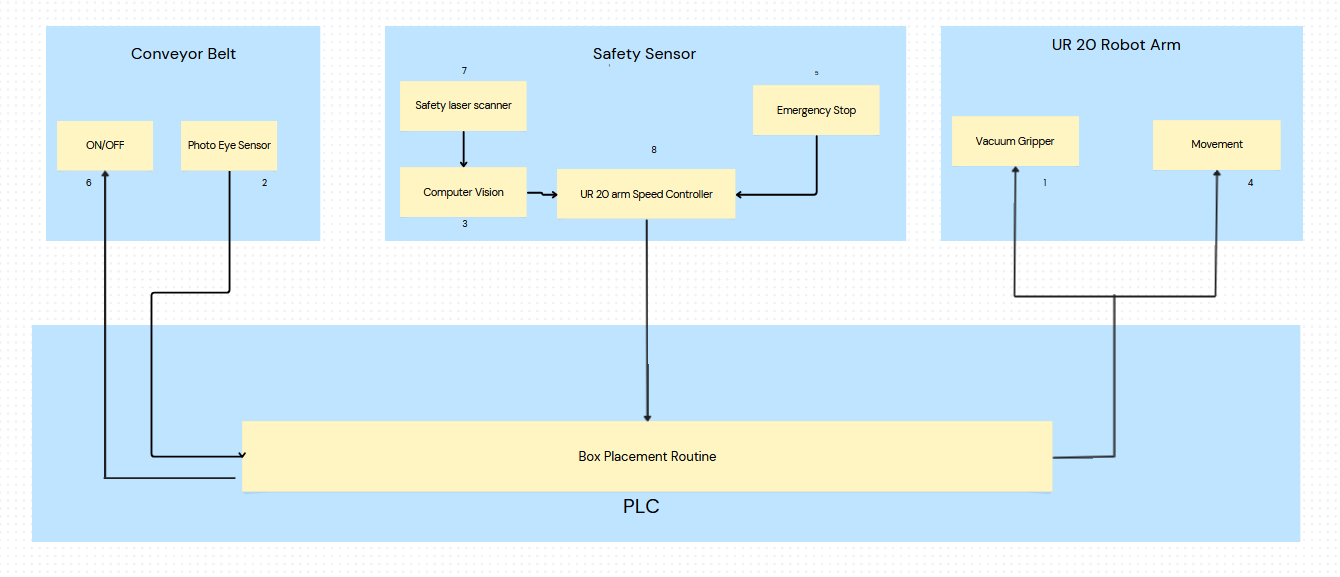
\includegraphics[width=0.90\textwidth]{images/dataflow.png}
 \caption{System architecture}
\end{figure}